








\begin{activite}[Modéliser une situation physique : système et objets]

Lorsqu'on étudie une situation physique dans laquelle plusieurs objets sont présents, on doit distinguer un objet en particulier qui nous intéresse. C'est cet objet que l'on étudie : on veut connaître sa position, sa vitesse, comment va évoluer son mouvement, etc. L'objet qu'on étudie est appelé le \textbf{système}.


\begin{minipage}{.48\linewidth}
\textbf{Apprenons à observer une situation} (image ci-contre). Nous sommes intéressé par le mouvement du skieur. Quels sont les objets en présence importants pour comprendre le mouvement du skieur ? Quel est le système étudié ?
\end{minipage}%
\hfill
\begin{minipage}{.48\linewidth}
\centering
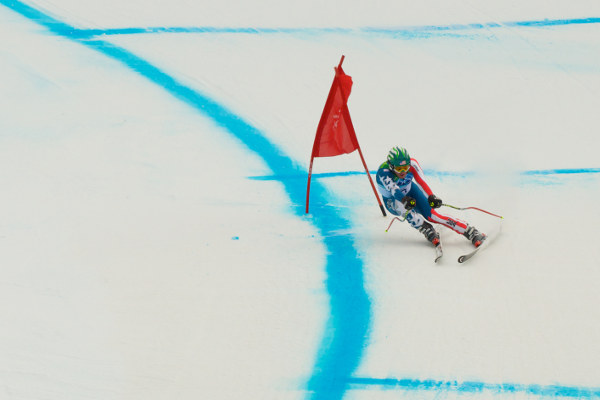
\includegraphics[width=.9\linewidth]{skieur} \\
{\scriptsize \textsl{Source : commons.wikimedia.org}} % https://commons.wikimedia.org/wiki/File:2010_Winter_Olympics_Bode_Miller_in_downhill.jpg#/media/File:2010_Winter_Olympics_Bode_Miller_in_downhill.jpg
\end{minipage}

\end{activite}










\begin{activite}[Action mécanique]


Lorsqu'un objet agit sur un autre objet, on parle d'\textbf{action mécanique}.

Si les deux objets se touchent, on dit qu'il y a \textbf{action mécanique de contact} (exemple : un homme qui pousse une armoire). Par contre, si les deux objets ne se touchent pas, on dit qu'il y a \textbf{action mécanique à distance} (ex : le Soleil qui attire la Terre).   

L'objet qui exerce l'action est appelé \textbf{acteur}. 

\vspace{1em}

\textsl{Voici quatre situations. Après les avoir observées, compléter le tableau suivant, en vous aidant de la question posée pour définir quel objet est l'acteur.}

\vspace{1em}

\begin{minipage}[c]{.2\linewidth}
\centering%
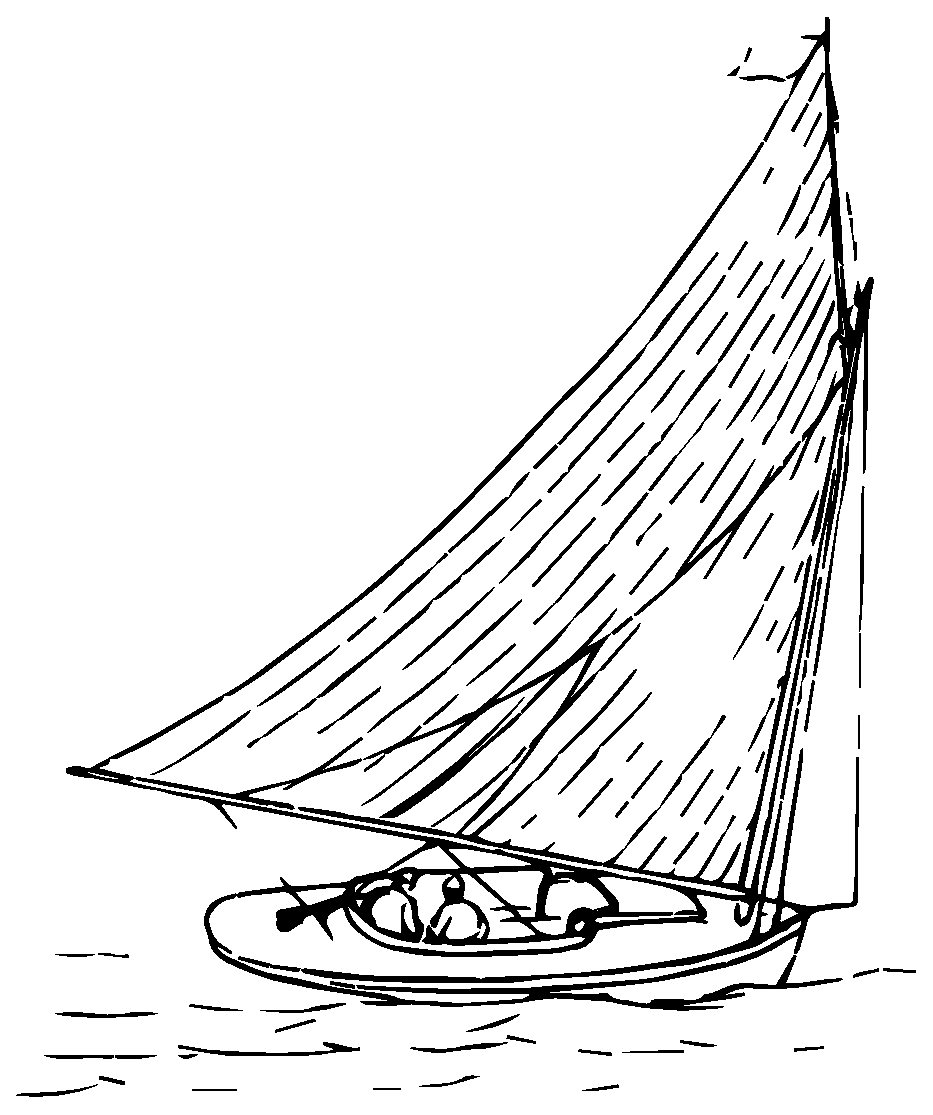
\includegraphics[angle=0,width=.5\linewidth]{bateau} 
% source : openclipart
\end{minipage}\hfill%
\begin{minipage}[c]{.26\linewidth}
\centering%
\includegraphics[angle=0,width=.7\linewidth]{billeSeule}
\end{minipage}\hfill%
\begin{minipage}[c]{.26\linewidth}
\centering%
\includegraphics[angle=0,width=.7\linewidth]{billeAimant}
\end{minipage}\hfill%
\begin{minipage}[c]{.2\linewidth}
\centering%
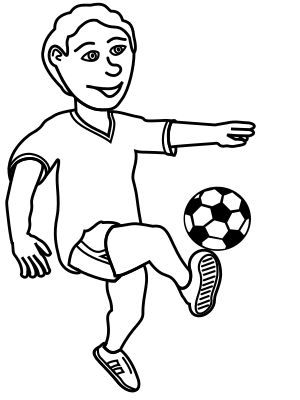
\includegraphics[angle=0,width=.3\linewidth]{footplayer}
% source : openclipart
\end{minipage}\\[.5em]
%
%
\begin{minipage}[c]{.2\linewidth}
\centering
\footnotesize{1 -- Pourquoi le bateau avance-t-il ?}  
\end{minipage}\hfill%
\begin{minipage}[c]{.26\linewidth}
\centering
\footnotesize{2 -- Pourquoi la bille descend-elle ?}
\end{minipage}\hfill%
\begin{minipage}[c]{.26\linewidth}
\centering
\footnotesize{3 -- Pourquoi la bille est-elle déviée ?}
\end{minipage}\hfill%
\begin{minipage}[c]{.2\linewidth}
\centering
\footnotesize{4 -- Pourquoi le ballon monte-t-il en l'air ?}
\end{minipage}

\vspace{1em}

\begin{center}
\renewcommand*\tabularxcolumn[1]{>{\centering\arraybackslash}m{#1}}
\begin{Ctableau}{\linewidth}{5}{c}
\hline
%Situation \no & \multicolumn{1}{c|}{1} & \multicolumn{1}{c|}{2} & \multicolumn{1}{c|}{3} & \multicolumn{1}{c|}{4} \\ \hline
Système & Bateau  & Bille & Bille & Ballon \\ \hline
Action & & & & \\ \hline
Acteur & & & & \\ \hline
Type d'action mécanique & & & & \\ \hline
\end{Ctableau}
\end{center}

\end{activite}

\newpage

\begin{activite}[Modélisation des actions mécaniques]

Les \textbf{actions mécaniques} sont \underline{modélisées} par des \textbf{forces} que l'on \underline{représentent} par un \textbf{vecteur} (donc une \og flèche \fg). Le but est de montrer par ce vecteur l'effet de l'action mécanique sur l'objet étudié.

\vspace{1em}


\begin{minipage}{.58\linewidth}
Voici une situation où un joueur exerce une action mécanique sur un ballon pour le lancer (figure ci-contre). On veut modéliser cette action mécanique par une force.

Quelles informations sont nécessaires pour décrire cette action ?



\end{minipage}%
\hfill
\begin{minipage}{.38\linewidth}
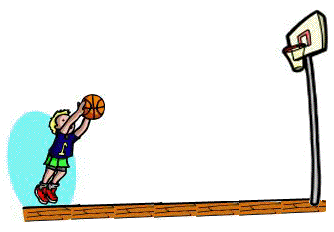
\includegraphics[width=.9\linewidth]{basketShoot}
\end{minipage}

Représenter sur la figure ci-dessus la force qu'exerce le joueur sur la ballon. On donne un nom à cette force, par exemple $\vect{F}_{\text{joueur}/\text{ballon}}$ (qu'on lit \og force du joueur sur le ballon \fg). Ajouter le nom de la force sur la figure.   

\end{activite}




\begin{activite}[Applications]

Pour les deux situations physiques ci-dessous, faire une analyse complète : objets en présence, système, description des actions mécaniques et représentation des forces par des vecteurs.

\vspace{1em}

\begin{minipage}[c]{.48\linewidth}
\centering%
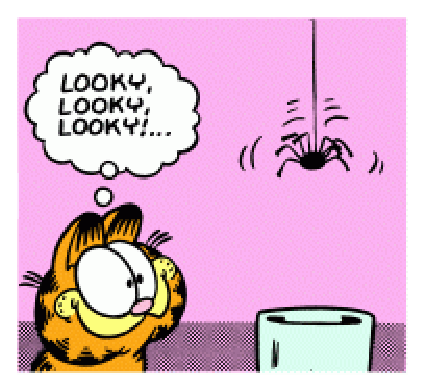
\includegraphics[angle=0,width=.5\linewidth]{garfieldAraignee}
\end{minipage}\hfill%
\begin{minipage}[c]{.48\linewidth}
\centering%
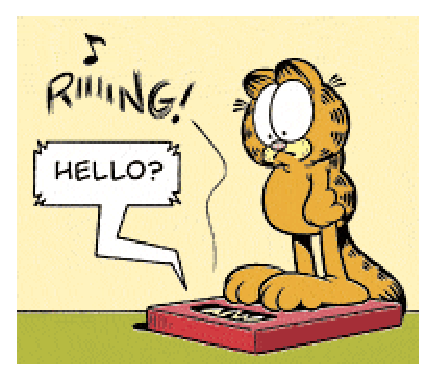
\includegraphics[angle=0,width=.5\linewidth]{garfieldBalance}
\end{minipage}\\[1em]
\begin{minipage}[c]{.48\linewidth}
On s'intéresse au mouvement de l'araignée.
\end{minipage}\hfill%
\begin{minipage}[c]{.48\linewidth}
On s'intéresse au mouvement de Garfield.
\end{minipage}

\end{activite}







\begin{activite}[Situations supplémentaires à étudier]


Pour les situations physiques ci-dessous, faire une analyse complète : objets en présence, système, description des actions mécaniques et représentation des forces par des vecteurs.

\vspace{1em}

\begin{minipage}[c]{.48\linewidth}
\centering%
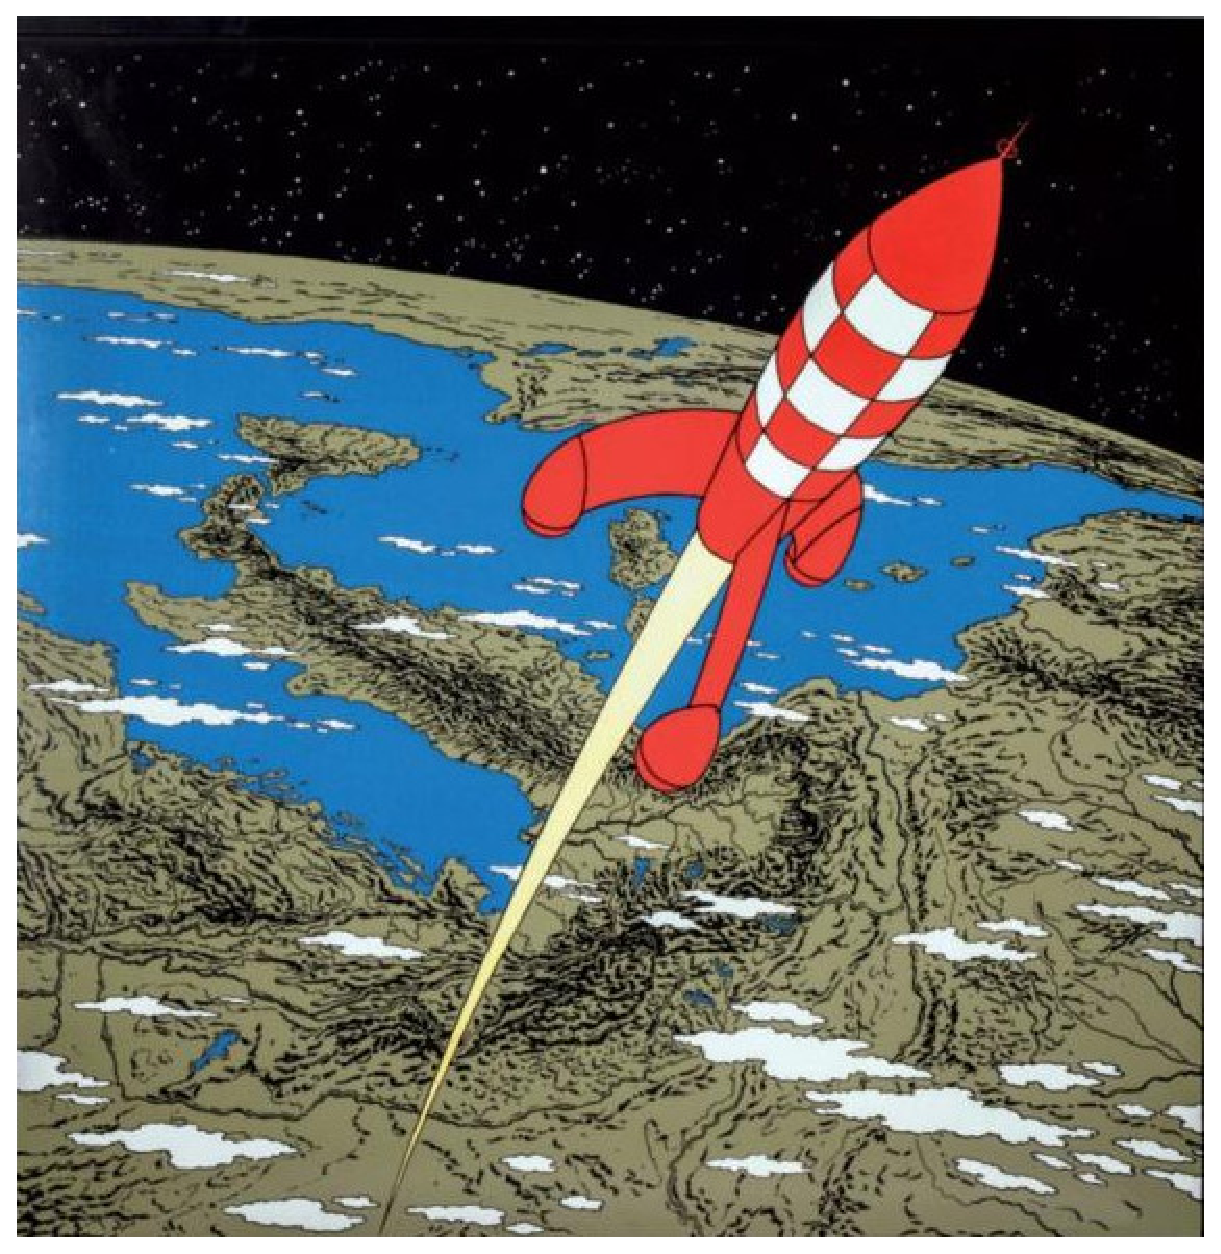
\includegraphics[angle=0,width=.5\textwidth]{tintinFusee}
\end{minipage}\hfill%
\begin{minipage}[c]{.48\linewidth}
On s'intéresse au mouvement de la fusée.
\end{minipage}\\[1em]



\begin{minipage}[c]{.48\linewidth}
\centering%
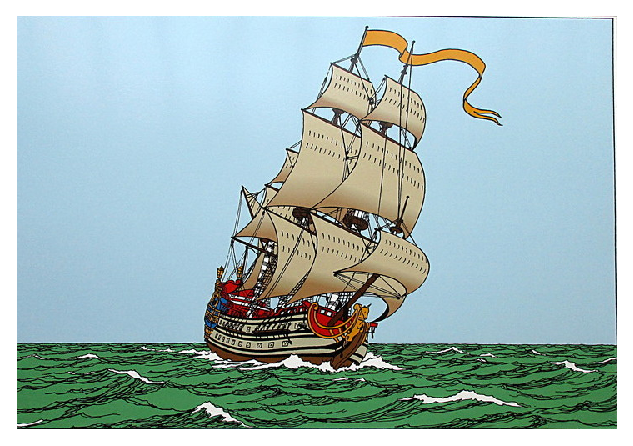
\includegraphics[angle=0,width=.65\textwidth]{tintinBateau}
\end{minipage}\hfill%
\begin{minipage}[c]{.48\linewidth}
On s'intéresse au mouvement du bateau.
\end{minipage}\\[1em]




\begin{minipage}[c]{.48\linewidth}
\centering%
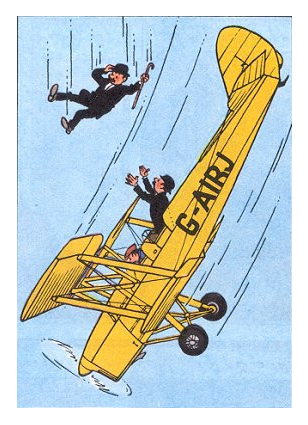
\includegraphics[angle=0,width=.45\textwidth]{tintinAvion}
\end{minipage}\hfill%
\begin{minipage}[c]{.48\linewidth}
On s'intéresse au mouvement de Dupont, puis dans un second temps à celui de l'avion.
\end{minipage}


\end{activite}



\begin{activite}[Les différents types de variables]

\begin{partie}[Les différents types de variables dans une expérience]

Dans une expérience, plusieurs variables entrent en jeu. Il y a toujours une \emph{variable indépendante} et une \emph{variable dépendante}, ainsi qu'un nombre plus ou moins grand de \emph{variables contrôlées}.   

\begin{itemize}
\item \textbf{variable indépendante} : c'est la variable, le paramètre, que l'on fait varier dans l'expérience (cause) ;
\item \textbf{variable dépendante} : c'est la variable, le paramètre, que l'on mesure dans l'expérience après chaque variation de la variable indépendante (effet) ;
\item \textbf{variables contrôlées} : ce sont les variables, les paramètres de l'expérience, qui doivent rester constants afin de ne pas fausser les résultats. 
\end{itemize}

Ainsi, l'expérimentateur modifie la variable indépendante, et regarde comment varie alors la variable dépendante (en la mesurant). Pendant tout le temps de l'expérience, l'expérimentateur vérifie que les variables contrôlées ne sont pas modifiées.
\end{partie}

\begin{partie}[Des cas pratiques pour s'entraîner]

Pour chacune des expériences décrites ci-dessous, identifier les variables indépendante, dépendante et éventuellement contrôlées choisies par l'expérimentateur.

\vspace{1em}

{\footnotesize 

\begin{minipage}[c]{.68\linewidth}
\textbf{Expérience 1 --} On souhaite étudier le lien entre l'intensité de la couleur, notée $A$ et la concentration, notée $C$, d'un sirop à la menthe. Pour cela, on utilise un appareil qui mesure l'intensité de lumière absorbée à travers une cuve contenant une solution de sirop à la menthe. Le but de cette expérience est de montrer que l'intensité de la couleur du sirop est proportionnelle à la concentration en sirop, donc que $A = k \times C$, où $k$ est une constante.
\end{minipage}\hfill%
\begin{minipage}[c]{.28\linewidth}
\centering
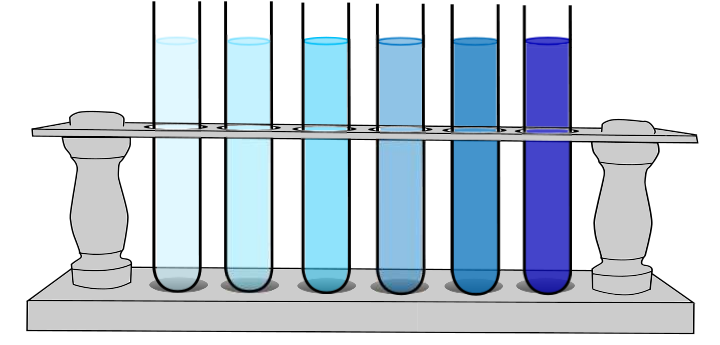
\includegraphics[angle=0,width=.6\linewidth]{echelle-teinte}
\end{minipage}


\vspace{2em}

\begin{minipage}[c]{.68\linewidth}
\textbf{Expérience 2 --}On souhaite étudier le lien entre la chaleur fournie, notée $Q$, à une casserole contenant un litre d'eau, et la variation de température $\Delta T$ de l'eau contenue dans la casserole. Pour cela, on utilise un brûleur à gaz qui permet de connaître la quantité de chaleur transmise, et un thermomètre que l'on place dans l'eau. Le but de cette expérience est de montrer que la température atteinte par l'eau est proportionnelle à la quantité de chaleur fournie, donc que $Q = k \times T$, où $k$ est une constante.
\end{minipage}\hfill%
\begin{minipage}[c]{.28\linewidth}
\centering
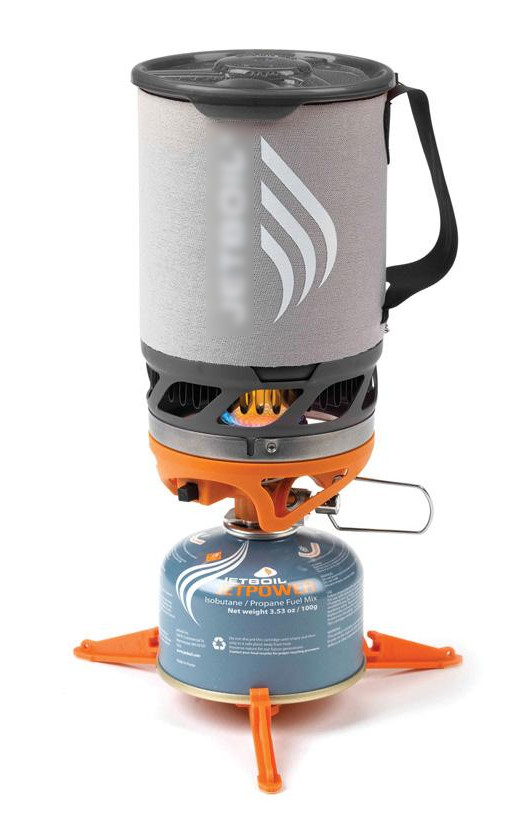
\includegraphics[angle=0,width=.3\textwidth]{jetboil}
\end{minipage}

\vspace{2em}

\begin{minipage}[c]{.68\linewidth}
\textbf{Expérience 3 --} On souhaite étudier le lien entre la tension $U$ aux bornes d'une résistance $R$  et l'intensité $I$ du courant électrique qui la traverse. Pour cela, on dispose d'un circuit électrique où on peut placer une résistance, d'un générateur réglable qui permet de choisir la tension $U$ appliquée aux bornes de la résistance, et d'un ampèremètre pour mesurer l'intensité du courant électrique circulant dans le circuit. Le but de cette expérience est de montrer que la tension aux bornes de la résistance est proportionnelle à l'intensité du courant électrique circulant dans la résistance, donc que $U = R \times I$.
\end{minipage}\hfill%
\begin{minipage}[c]{.28\linewidth}
\centering
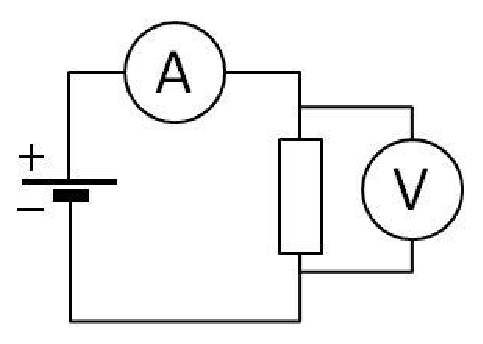
\includegraphics[angle=0,width=.6\linewidth]{resistance}
\end{minipage}

}% fin du footnotesize

\end{partie}
\end{activite}

